% =====================================================================
%  Project 10: Teaching an Agent to Imagine
%  SJTU — AI / Deep Learning & Reinforcement Learning, final project
% =====================================================================
\documentclass[11pt]{article}

\usepackage[utf8]{inputenc}
\usepackage[T1]{fontenc}
\usepackage{amsmath,amssymb}
\usepackage{graphicx}
\usepackage{booktabs}
\usepackage{caption}
\usepackage{geometry}
\geometry{a4paper, margin=1in}
\usepackage{xcolor}
\usepackage[colorlinks=true, linkcolor=blue, citecolor=blue, urlcolor=blue]{hyperref}

% Light note box for parts still to be completed by the author.
\newcommand{\todo}[1]{\medskip\noindent\fbox{\parbox{0.97\linewidth}{%
  \textit{\textbf{[Author note / to be completed]}}\\ #1}}\medskip}

\graphicspath{{../results/}}

\title{Teaching an Agent to Imagine:\\
       Learning a World Model to Accelerate Dyna-Q in a Noisy GridWorld}
\author{% TODO: your name / student ID
        Fei Xuemin (523202910009)}
\date{\today}

\begin{document}
\maketitle

% =====================================================================
\section{Introduction}\label{sec:intro}
% Target: 200–300 words. Draft below — rewrite in your own voice.
We study whether a neural network that predicts an environment's next state
can make a reinforcement-learning agent learn faster, and what happens when
that predictor is wrong. The testbed is a noisy $8\times8$ GridWorld
(20\% action noise). We learn a \emph{world model} (a transition network and a
reward network) from random-policy experience, freeze it, and use it to
generate ``imagined'' experience for Dyna-Q. We compare Dyna-Q ($K{=}10$)
against tabular Q-learning ($K{=}0$, the no-model baseline) and Value Iteration
(the oracle ceiling, computed from the true transition probabilities). The
central question (Lec.~17--21): does a learned model improve sample efficiency,
and how does model quality govern that benefit?



% =====================================================================
\section{Environment}\label{sec:env}
% Target: 250–350 words.
The environment is a deterministic-topology, stochastic-dynamics GridWorld.
States are integer coordinates $(r,c)$ with $r,c\in\{0,\dots,7\}$ (64 states),
start $(0,0)$, goal $(7,7)$, and 10 fixed wall cells; a BFS check guarantees a
start-to-goal path. Actions are $\{0{=}\text{up},1{=}\text{down},
2{=}\text{left},3{=}\text{right}\}$. With probability $0.8$ the intended action
is executed; with probability $0.2$ a uniformly random direction replaces it.
Bumping a wall or boundary leaves the agent in place. The reward is $+1.0$ on
reaching the goal (episode ends), and $-0.01$ per step otherwise; episodes time
out after 100 steps. The 20\% noise is essential: a deterministic environment
would make the world model a trivial lookup table, whereas noise forces it to
learn a genuine probability distribution and gives the imagined experience room
to help (or to mislead).

Figure~\ref{fig:fig1} shows the state-visitation heatmap of 100 random-policy
episodes: the top-left start region is visited far more than the bottom-right
goal region, confirming the dynamics behave as intended.

\begin{figure}[h]
  \centering
  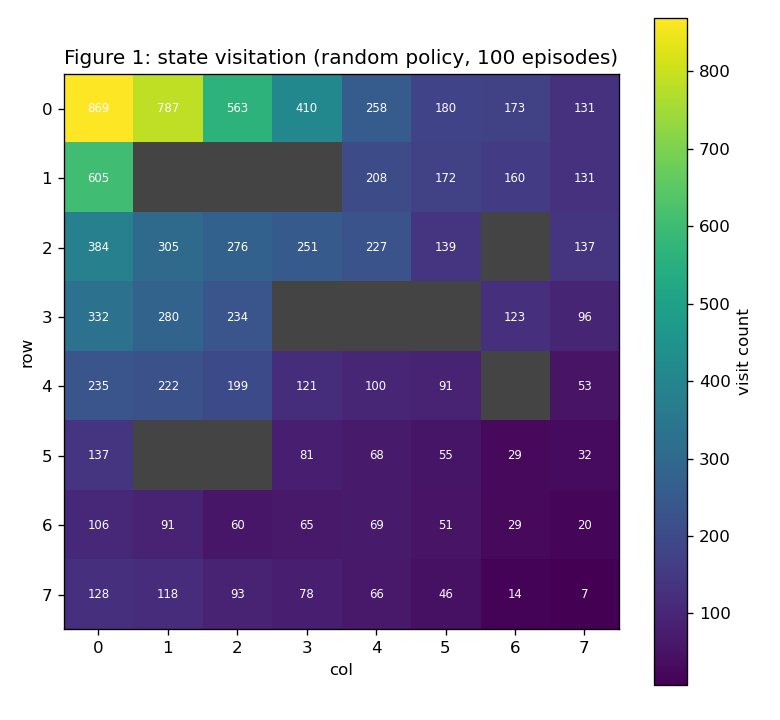
\includegraphics[width=0.55\linewidth]{figure1_visitation.png}
  \caption{\textbf{Figure 1.} State-visitation counts over 100 random-policy
  episodes. Walls are gray. Visitation decays smoothly from the start $(0,0)$
  to the rarely-reached goal $(7,7)$, verifying the environment.}
  \label{fig:fig1}
\end{figure}

The gradient is a direct read-out of the dynamics: every episode starts at
$(0,0)$, so the start region accumulates visits before the random walk has had
time to diffuse; the goal $(7,7)$ is an absorbing terminal that ends the episode
on contact, so it is reached rarely and never accumulates. The walls carve out
the low-count channels in between.

% =====================================================================
\section{World Model}\label{sec:wm}
% Target: 350–450 words.
We collect 10{,}000 transitions $(s,a,s',r)$ under a \emph{random} policy (so
the dataset covers the whole state space, not only an optimal path) and split
80/20 into train/validation. Each $(s,a)$ is encoded as the concatenation of a
64-dim state one-hot and a 4-dim action one-hot (68-dim input).

\paragraph{Transition network (classification).}
$68 \to 256 \to 256 \to 64$ logits over the next state, trained with
cross-entropy for 20 epochs (Adam). It predicts a \emph{distribution} over the
64 possible next states.

\paragraph{Reward network (regression).}
$68 \to 128 \to 64 \to 1$, trained with MSE for 20 epochs. Reward is easy to
learn (almost always $-0.01$; only entering the goal gives $+1.0$); the
validation MSE reaches $\approx 9\times10^{-5}$.

Figure~\ref{fig:fig2} (left) plots validation accuracy versus epoch; (right)
lists top-3 predicted next states for five probe $(s,a)$ pairs, all physically
plausible (within one step of the queried cell).

\paragraph{Why accuracy plateaus below 100\% (and slightly above the 75--85\%
band).}
The transition accuracy plateaus at $\approx 87\%$, not $100\%$, and this is a
property of the environment, not a model defect. Under 20\% noise the intended
direction is realized with probability $0.8 + 0.2\cdot\tfrac14 = 0.85$, so a
\emph{perfect} mode predictor scores about $0.85$ on open-grid cells. Near walls
and boundaries several directions collapse onto the \emph{same} next cell (a
wall bump keeps the agent in place), so the most-likely next state can carry
probability $0.90+$; e.g.\ the probe ``$(0,0)$, up'' predicts staying at $(0,0)$
with $p\approx0.91$. Because the random policy over-samples the wall-dense
top-left region, the dataset-averaged ceiling sits a little above $0.85$, which
is why our model lands at $\approx 87\%$ rather than inside the nominal
$75\text{--}85\%$ band. The gap to $100\%$ is exactly the irreducible noise
entropy: the 20\% of steps whose direction is randomized are inherently
unpredictable.

\begin{figure}[h]
  \centering
  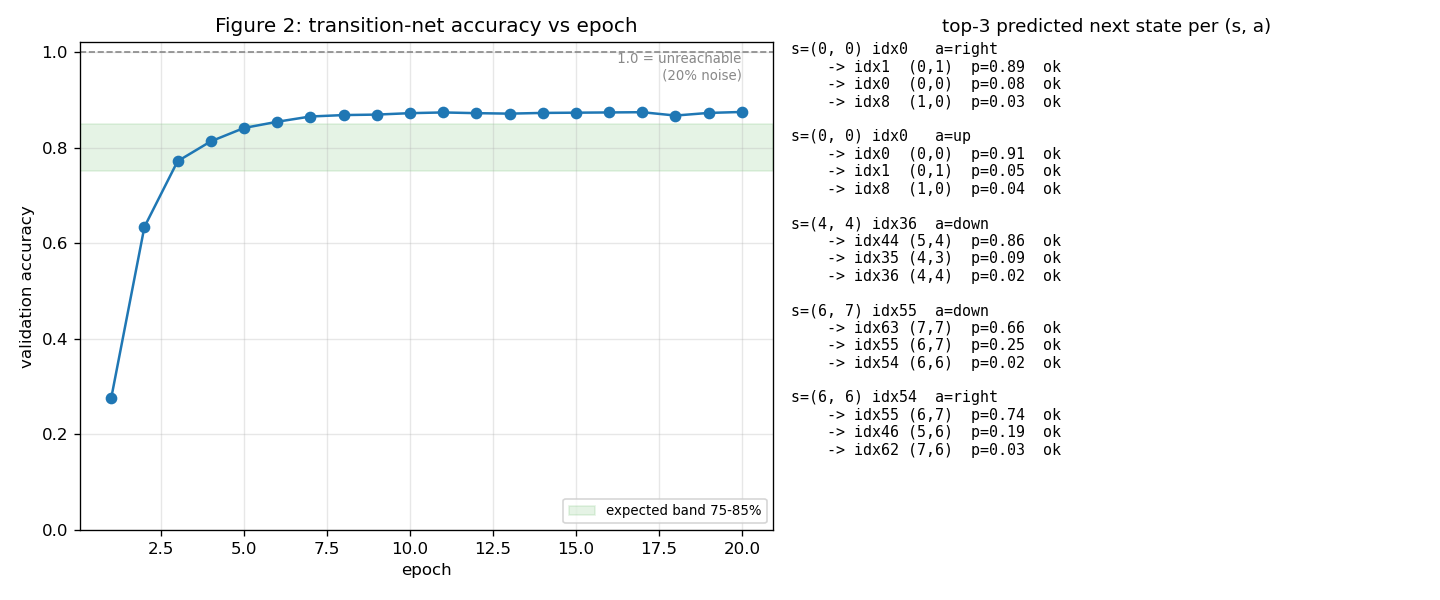
\includegraphics[width=\linewidth]{figure2_transition_accuracy.png}
  \caption{\textbf{Figure 2.} Left: transition-network validation accuracy vs
  epoch; the shaded band is the nominal 75--85\% expectation and the dashed line
  marks the unreachable 100\% (capped by 20\% noise). Right: top-3 predicted
  next states for five $(s,a)$ probes; each is within one step of the queried
  cell (``ok''), confirming the predictions are physically sensible.}
  \label{fig:fig2}
\end{figure}

% =====================================================================
\section{Dyna-Q Algorithm}\label{sec:dynaq}
% Target: 300–400 words.
Dyna-Q maintains a tabular $Q\in\mathbb{R}^{64\times4}$. After each real
environment step it performs one real Q-learning update and then $K{=}10$
imagined updates using the frozen world model, all with the same Bellman target
\[
  Q(s,a) \leftarrow Q(s,a) + \alpha\big[r + \gamma\max_{a'}Q(s',a') - Q(s,a)\big].
\]
Three design choices (to be justified against Lec.~17/19/21):
\begin{enumerate}
  \item Imagined $(s,a)$ are sampled only from \emph{previously visited} pairs in
  the replay buffer — never from states the model has not seen, where its
  predictions are unreliable.
  \item The world model is trained and \emph{frozen} before RL begins; its
  weights never update during RL, isolating the pure effect of the model.
  \item Baseline ${}=$ Dyna-Q($K{=}0$) (no model); ceiling ${}=$ Value Iteration
  on the true $P[s,a,s']$ from \texttt{get\_all\_transitions()}.
\end{enumerate}

Each choice matters for a concrete reason. (1) Sampling imagined $(s,a)$ only
from visited pairs keeps imagination inside the model's support: a neural model
queried on a state--action it never saw returns an essentially arbitrary
next-state distribution, and a Bellman backup on that garbage target would
corrupt $Q$ rather than refine it. (2) Freezing the model isolates the variable
under study --- if the model kept learning during RL we could not attribute a
speed-up (or a slow-down) to the \emph{model} as opposed to ongoing model
improvement. (3) Dyna-Q($K{=}0$) and Value Iteration bracket the result from
below and above: the former is the same algorithm with the imagination loop
switched off (so any difference is purely the model's effect), and the latter is
the exact optimum from the true $P[s,a,s']$, telling us how much head-room
remains.

% =====================================================================
\section{Main Experiment Results}\label{sec:results}
% Target: 500–700 words.
\begin{figure}[h]
  \centering
  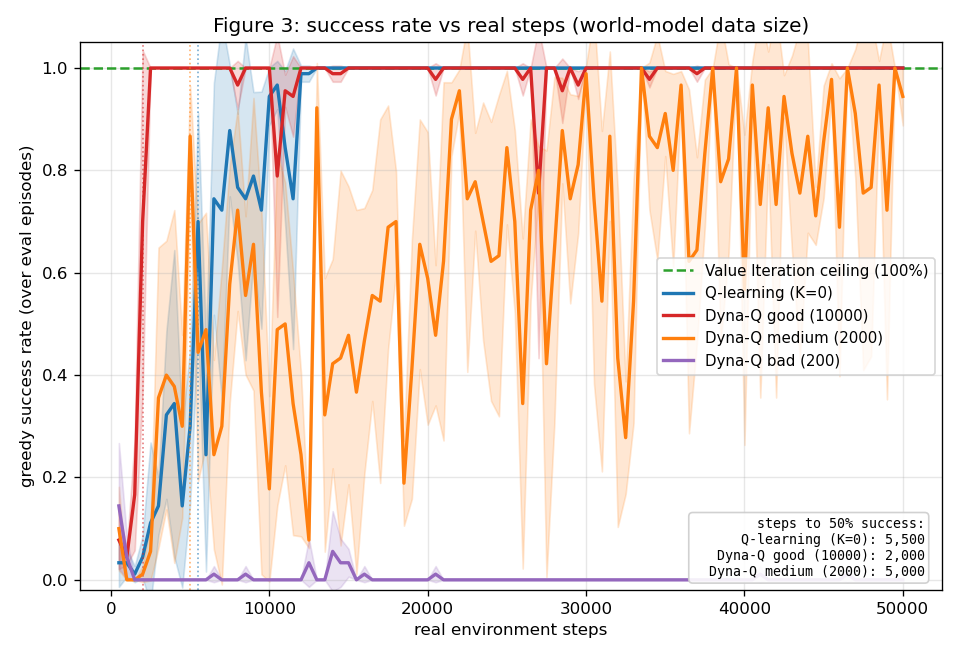
\includegraphics[width=0.75\linewidth]{figure3_learning_curves.png}
  \caption{\textbf{Figure 3.} Greedy success rate vs real environment steps
  (mean $\pm 1$ std, 3 seeds): Value Iteration ceiling (dashed), Q-learning
  ($K{=}0$), and Dyna-Q ($K{=}10$) with world models trained on 10{,}000 (good),
  2{,}000 (medium) and 200 (bad) transitions. The good model accelerates
  learning; the bad model collapses to $0\%$ (Section~\ref{sec:failure}).}
  \label{fig:fig3}
\end{figure}
\begin{figure}[h]
  \centering
  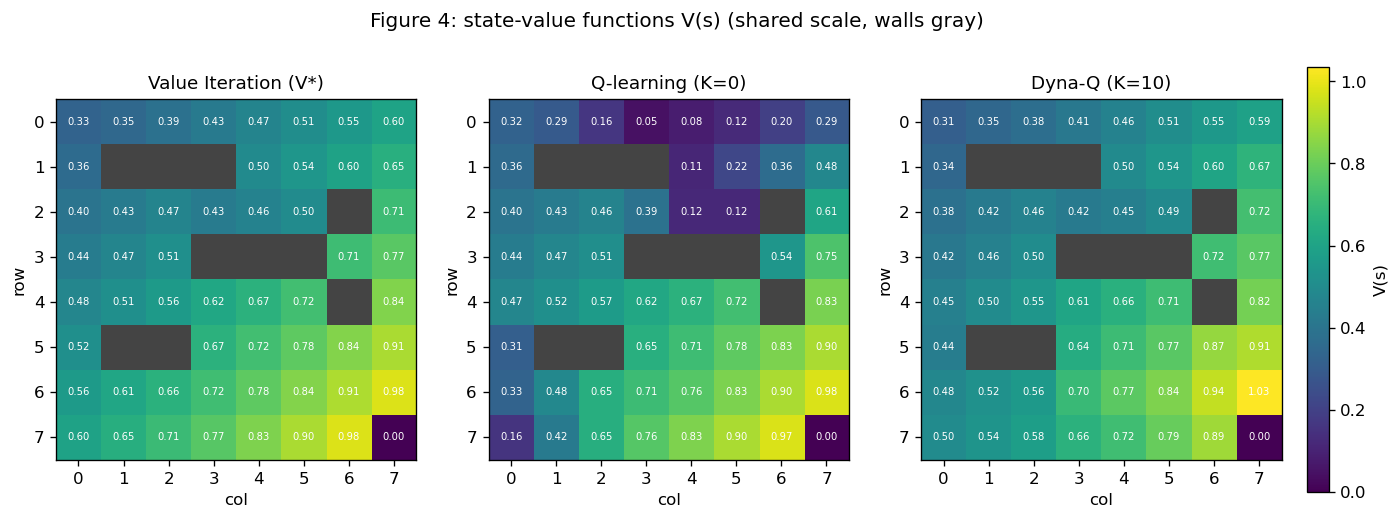
\includegraphics[width=\linewidth]{figure4_value_heatmaps.png}
  \caption{\textbf{Figure 4.} Value-function heatmaps (VI / Q-learning / Dyna-Q),
  shared color scale, walls in gray.}
  \label{fig:fig4}
\end{figure}

\paragraph{(1) Does Dyna-Q learn faster than Q-learning?}
Yes, dramatically, in the early regime. Reading Figure~\ref{fig:fig3}, Dyna-Q
($K{=}10$, good model) first reaches $50\%$ greedy success at $\approx2{,}000$
real steps versus $\approx5{,}500$ for $K{=}0$ ($\approx2.7\times$ faster), and
$90\%$ at $\approx2{,}500$ versus $\approx10{,}000$ steps ($4\times$). The gap is
starkest very early: at $2{,}000$ real steps Dyna-Q already averages $70\%$
success while $K{=}0$ sits at $4\%$. So the benefit is overwhelmingly one of
\emph{sample efficiency}, not of a higher final score.

\paragraph{(2) Do both converge to the Value-Iteration ceiling?}
Yes. Both reach $100\%$ greedy success (Dyna-Q by $\approx13$K steps, $K{=}0$ by
$\approx20$K) and sit on the dashed VI ceiling thereafter. The state values agree
too: $V(\text{start})$ is $0.330$ for VI, $0.325$ for $K{=}0$ and $0.314$ for
$K{=}10$ --- a negligible residual gap from finite $\varepsilon$-greedy
exploration and sampling, not a structural one. The learned model changes
\emph{when} the optimum is reached, not \emph{whether}.

\paragraph{(3) What do the value heatmaps reveal (Figure~\ref{fig:fig4})?}
All three $V(s)$ fields share the same structure: value is highest at the goal and
decays smoothly outward, routed around the gray walls. The two learned agents
reproduce VI's gradient closely, confirming that Q-learning and Dyna-Q both
recover the optimal value-to-go; the only visible differences are mild
under-estimation in rarely-visited corners, which matters little for the greedy
policy.

\paragraph{(4) How does imagined experience change the early-learning regime?}
Each real step triggers $K{=}10$ Bellman backups on previously-visited $(s,a)$
pairs, so the goal's value is propagated backward many cells \emph{per real step}
rather than one. This is why Dyna-Q's curve rises almost vertically once the goal
is first found, while $K{=}0$ must physically traverse each transition to move
value one step back. The model effectively recycles real experience into many
extra planning sweeps (cf.\ Value Iteration), front-loading the learning.

\paragraph{(5) Where does the 20\% noise show up?}
In three places: the optimum itself is stochastic --- $V(\text{start})\approx0.33$
rather than near $1$, because noise lengthens trajectories and each step costs
$-0.01$; the per-seed bands in Figure~\ref{fig:fig3} are widest early (e.g.\
Dyna-Q is $0.70\pm0.33$ at $2{,}000$ steps), reflecting how much the first
goal-hit depends on lucky noise; and the curves stay slightly jagged even after
convergence because greedy evaluation is itself run in the noisy environment.

% =====================================================================
\section{Failure Analysis}\label{sec:failure}
% Target: 500–700 words.
\begin{figure}[h]
  \centering
  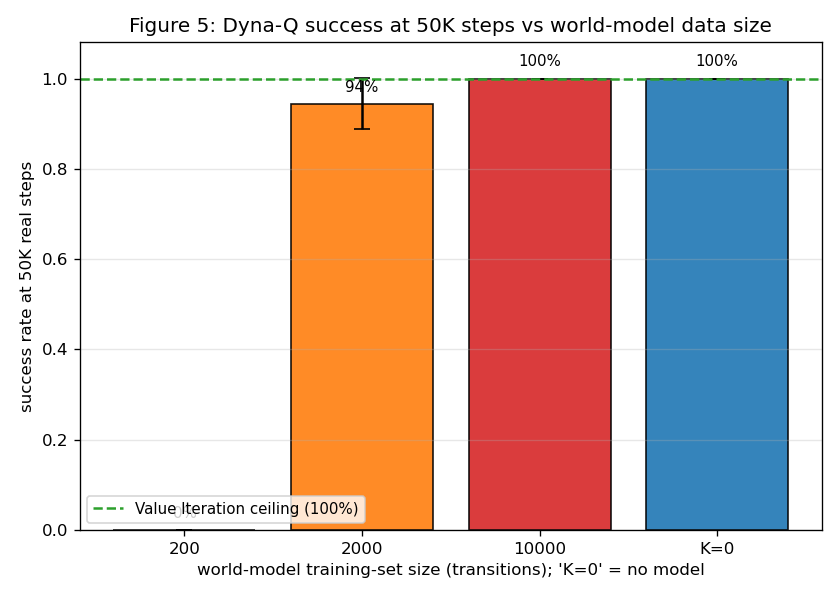
\includegraphics[width=0.6\linewidth]{figure5_data_scaling.png}
  \caption{\textbf{Figure 5.} Greedy success rate at 50K real steps vs
  world-model training-set size (200 / 2000 / 10{,}000 transitions) and the
  $K{=}0$ baseline (mean $\pm 1$ std, 3 seeds). The 200-transition model is the
  only condition that fails, and it fails completely.}
  \label{fig:fig5}
\end{figure}

\paragraph{Pre-registered prediction.}
Before running, I predicted (timestamped in
\texttt{report/p5\_prediction\_2026-06-15.md}) that the 200-transition model would
\emph{hurt}: its imagined Bellman targets would be wrong and, outnumbering the
real updates $10{:}1$, would drag Dyna-Q \emph{below} the $K{=}0$ baseline,
possibly plateauing under $100\%$. I predicted the 2000-transition model would
recover most of the speed-up, and that the data-scaling would be a
\emph{threshold} (2000 $\approx$ 10000, while 200 ``falls off a cliff'') rather
than smooth. The experiment confirmed all three.

\paragraph{What happened.}
Validation accuracy of the transition net drops from $\approx87\%$ (10{,}000
transitions) to $\approx80\%$ (2000) to $\approx7.5\%$ (200) --- the last barely
above the $1/64\approx1.6\%$ chance level. Plugged into Dyna-Q, the resulting
50K-step success rates (Figure~\ref{fig:fig5}) are $100\%$ (10{,}000), $94\%$
(2000), and $\mathbf{0\%}$ (200), against $100\%$ for $K{=}0$. The bad-model curve
in Figure~\ref{fig:fig3} never leaves the floor: it is not merely slow, it is
\emph{worse than using no model at all}.

\paragraph{Mechanism (Lec.~18/19/21).}
A Dyna-Q backup $Q(s,a)\leftarrow Q(s,a)+\alpha[\,r+\gamma\max_{a'}Q(s',a')-Q(s,a)\,]$
is only as good as the $(s',r)$ it is fed. The 200-transition model has seen each
$(s,a)$ at most a handful of times, so its softmax over next states is close to
uniform/wrong even for the visited pairs that imagination samples; the reward head
is similarly off (val.\ MSE $\sim\!2.5\times10^{-2}$ vs $\sim\!10^{-4}$ for the
good model). Each real step then applies one \emph{correct} update and ten
\emph{wrong} ones, so the wrong targets dominate by $10{:}1$ and push $Q$ toward a
spurious fixed point unrelated to $V^*$. The greedy policy read off this poisoned
$Q$ wanders and times out --- hence $0\%$. This is the same lesson as bootstrapping
on a bad function approximator: imagined experience is a multiplier, and it
multiplies error just as readily as signal.

\paragraph{Threshold, not gradient.}
The scaling is sharply non-linear. Going from 2000 to 10{,}000 transitions buys
almost nothing ($94\%\!\to\!100\%$), but going from 2000 down to 200 collapses the
agent entirely ($94\%\!\to\!0\%$). There is effectively a \emph{quality threshold}:
once the model is accurate enough that its imagined targets point, on average, the
right way, Dyna-Q tolerates the residual error and even benefits; below that
threshold the imagined updates are anti-correlated with the truth and the model
becomes actively destructive. Notably the same poisoning mechanism reappears in
Section~\ref{sec:innovation} under \emph{distribution shift}: a perfectly good
model, transplanted to an unseen map, supplies systematically wrong $(s',r)$ and
likewise drags Dyna-Q below the model-free baseline --- a bad model and a
good-but-misapplied model fail for the same reason.

% =====================================================================
\section{Innovation: An Improved World Model with a Local Field-of-View}\label{sec:innovation}

\paragraph{Motivation: a world model should learn the \emph{rules} of the world.}
The purpose of a world model is to capture the laws that govern an environment.
In this GridWorld those laws are simple and local: \emph{you cannot walk through
walls, and you must look at the road ahead}. Read this way, the model's real job
is to give the actor a pair of \emph{eyes}. The baseline transition network has
no eyes --- its only input is a 64-dim one-hot of the \emph{absolute} cell index,
which says nothing about what surrounds the agent. It can therefore do nothing
but \emph{memorize}, cell by cell, where each action leads on this particular
map. I hypothesized that a model that could instead \emph{see} its surroundings
might learn a position-invariant rule (``a wall to my right means moving right
keeps me in place'') and thereby generalize.

\paragraph{Input/output design.}
The improved world model augments the absolute anchor with a local field of view:
\[
  \text{obs} \;=\; \underbrace{\text{one-hot}(s)}_{64}\ \Vert\
  \underbrace{\text{window}_{3\times3}(s)}_{9}, \qquad
  \text{input} = \text{obs}\ \Vert\ \text{action}\ (77\text{-dim}),
\]
where the centered $3\times3$ window marks each surrounding cell $-1$ (wall or
off-grid), $+1$ (goal), or $0$ (free). Crucially, the network predicts the
\emph{entire next observation} $\text{obs}'$ --- the next state as a 64-way
classification \emph{and} the next $3\times3$ window --- plus the reward. That is,
it must predict not only \emph{where} it lands but how its local view of the
world \emph{transforms} as it moves.

\paragraph{A dropout data method to force the model to use its eyes.}
On a single static map the window is a deterministic function of position, hence
\emph{redundant} given the one-hot: a loss-minimizing network has no incentive to
read the window and will simply lean on the absolute index. To break this, I
randomly \emph{drop} (zero out) the one-hot block and/or the window block,
independently, for each training sample (probability $p$ each), so the network
must predict from whichever modality survives. I then evaluate under three
conditions: \emph{full}, \emph{state-only} (window dropped) and \emph{window-only}
(state dropped). Figure~\ref{fig:improved} shows the effect: with $p{=}0$ the
model co-adapts and collapses if either block is removed, whereas with $p{=}0.5$
it predicts the next state from the one-hot alone (state-only $0.87$) \emph{and}
from the window alone (window-only $0.73$). The window-only number is strikingly
high because, with boundaries and walls, most cells have a near-\emph{unique}
$3\times3$ ``fingerprint'' from which the model can recover its position.

\begin{figure}[h]
  \centering
  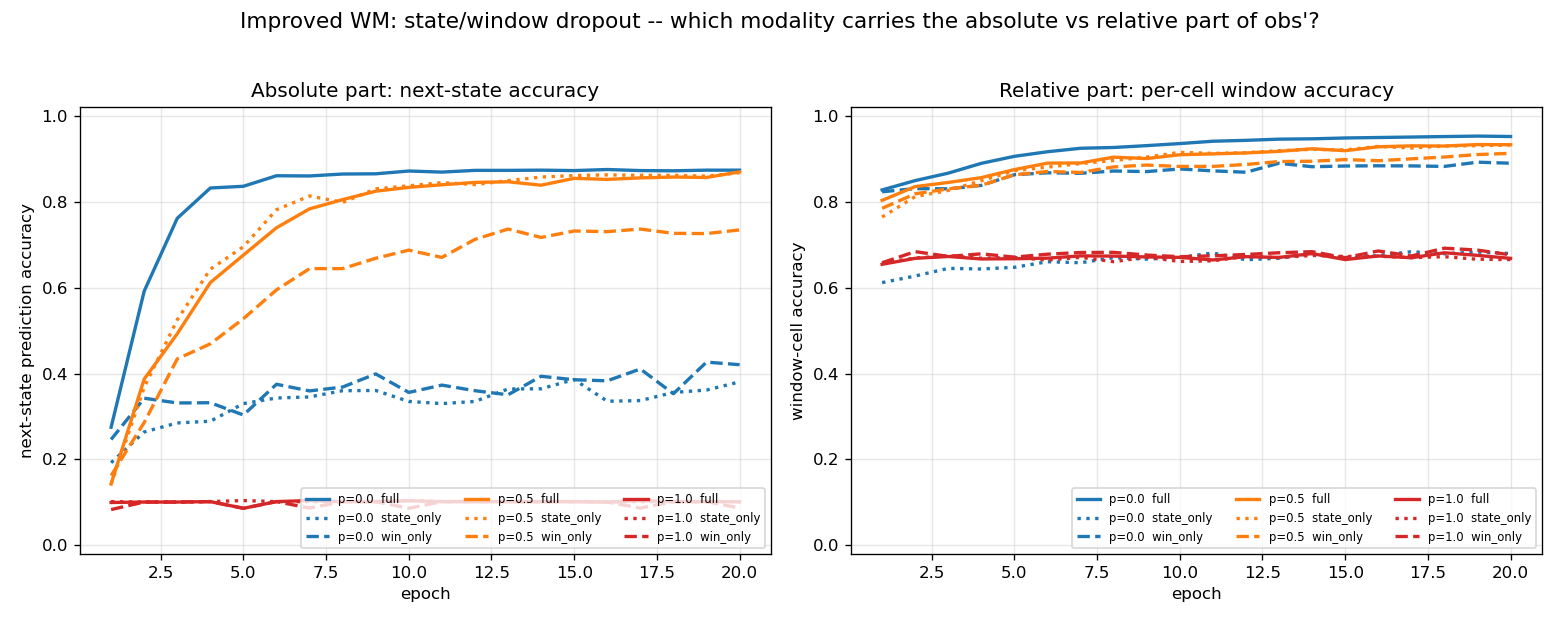
\includegraphics[width=\linewidth]{figure_improved_wm.png}
  \caption{\textbf{Figure 6.} Improved world model under anchor/window dropout.
  Left: next-state accuracy; right: per-cell window accuracy. Colour is the
  dropout probability $p$, line style the evaluation condition. With $p{=}0.5$
  both modalities independently support prediction; with $p{=}0$ the model
  collapses when either is removed.}
  \label{fig:improved}
\end{figure}

\paragraph{Same map: as good, and no better.}
Plugged into Dyna-Q on the training map (Figure~\ref{fig:ablation}, green), the
improved model converges to the optimum exactly like the one-hot model and the
cheaper tabular/replay variants --- all reach $100\%$. This is the central honest
finding: \textbf{this task is, at bottom, a ``memorize-the-map'' problem.} On a
single fixed, fully observable map, tabular Dyna-Q (indeed plain Q-learning)
already attains the Value-Iteration optimum; it is effectively as good as
anything can be, so a learned world model is \emph{redundant} and cannot beat
Dyna-Q. Its worth in this project is pedagogical --- a vehicle for understanding
what a world model is, fundamentally a study of an RL methodology.

\begin{figure}[h]
  \centering
  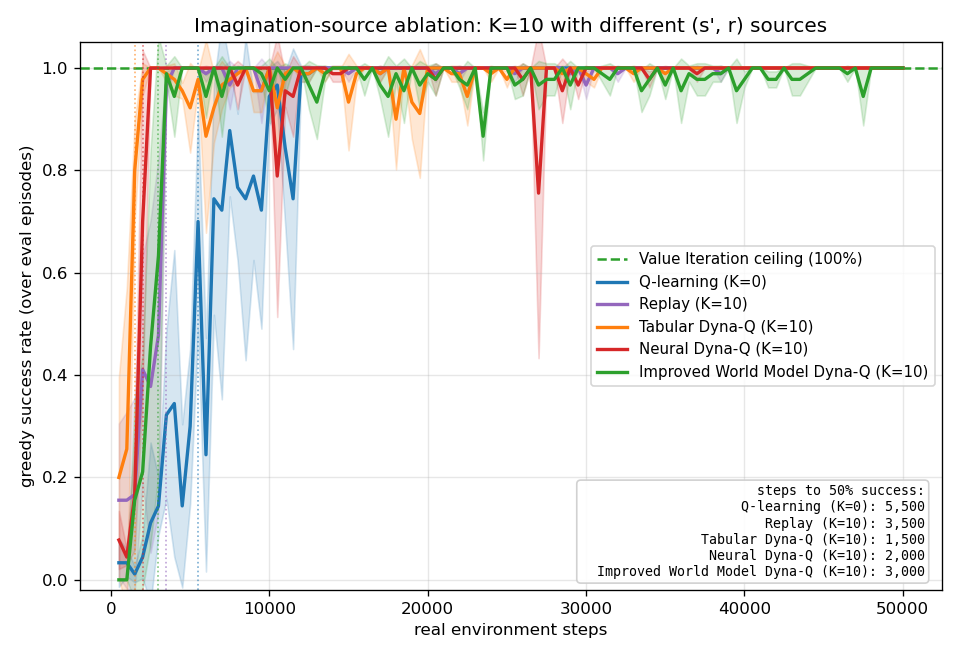
\includegraphics[width=0.7\linewidth]{figure_ablation_imagination.png}
  \caption{\textbf{Figure 7.} Same training map: imagination-source ablation with
  the improved world model added (green). All variants reach the Value-Iteration
  ceiling; the world model gives no advantage over tabular imagination here.}
  \label{fig:ablation}
\end{figure}

\paragraph{New map: why the idea cannot succeed \emph{in this project}.}
The true test of ``eyes'' is generalization. I froze both world models (trained
on the original map) and dropped them onto a \emph{new}, unseen wall layout (same
start and goal; Figure~\ref{fig:newmap}, left), then ran Dyna-Q without
retraining. Figure~\ref{fig:newmap} reports the result. Value Iteration and
tabular Dyna-Q --- which use the new map's \emph{own} dynamics --- reach $100\%$,
but \emph{both frozen world models collapse} ($\sim$0--10\%), and the improved
model is \textbf{not} better than the one-hot baseline. Two mechanisms combine.
First, both models predict the \emph{absolute} next state, which is inherently
map-specific; transplanted to a new map they replay the \emph{old} map's
transitions and actively \emph{poison} the Q-table --- which is why they fall
\emph{below} the no-transfer tabular agent (the same failure as a bad model in
the failure analysis, now triggered by distribution shift). Second, because the
improved model was trained on a \emph{single static map}, the window was
redundant with the one-hot, so it never had a reason to learn a transferable rule
from it; on the new map the pair (old-map one-hot, new-map window) is an
\emph{out-of-distribution} combination the network never saw, so the extra
window input perturbs rather than rescues the prediction.

\begin{figure}[h]
  \centering
  \begin{minipage}{0.40\linewidth}\centering
    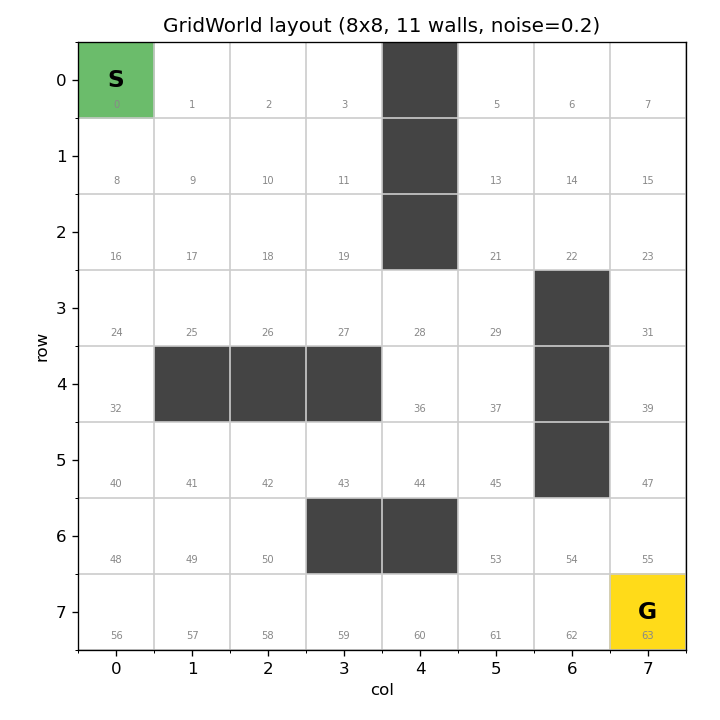
\includegraphics[width=\linewidth]{newmap_layout.png}
  \end{minipage}\hfill
  \begin{minipage}{0.58\linewidth}\centering
    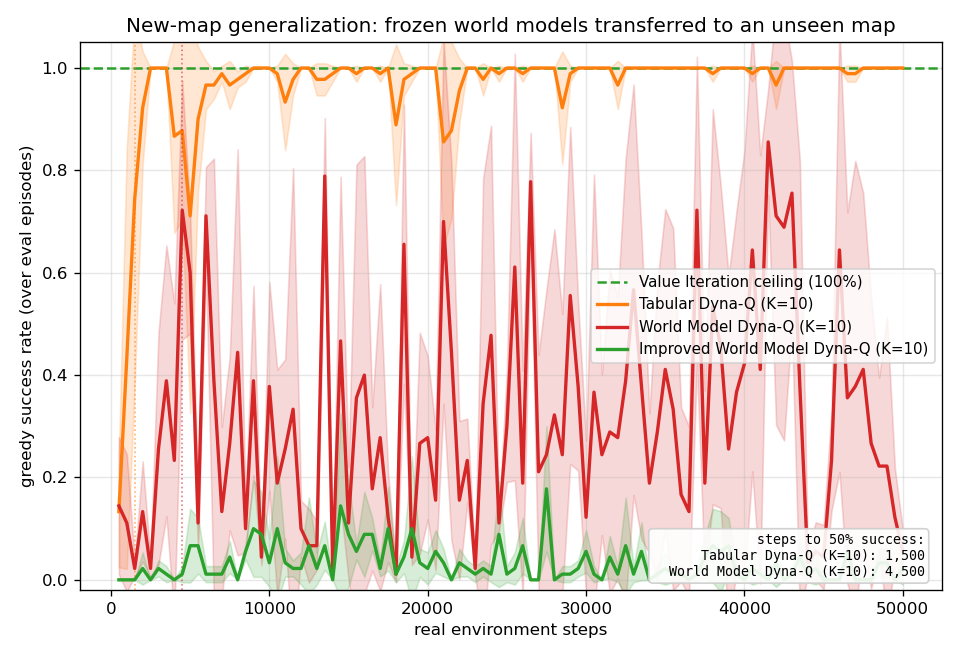
\includegraphics[width=\linewidth]{figure_newmap_generalization.png}
  \end{minipage}
  \caption{\textbf{Figure 8.} Generalization to an unseen map. Left: the new
  wall layout (start green, goal gold). Right: with the world models frozen from
  the \emph{old} map, Value Iteration and tabular Dyna-Q solve the new map
  ($100\%$), while both frozen world models collapse and even fall below the
  model-free tabular agent; the improved model is no better than the one-hot one.}
  \label{fig:newmap}
\end{figure}

This exposes the fundamental limitation: \textbf{the idea is essentially
impossible to realize within this project, because the data are static} --- one
fixed map, fixed walls. However the model is trained, it can only rote-memorize
this single map; there is no \emph{distribution of maps} from which a transferable
``don't-walk-through-walls'' rule could be learned. Genuinely giving the actor
eyes would require (i) training across \emph{many} maps so the local view is no
longer redundant, and (ii) a \emph{relative} output (a displacement $\Delta$,
applied as $s'=s+\Delta$) that is map-invariant --- both outside the static,
single-map setting of this assignment.

% =====================================================================
\section{Reflection}\label{sec:reflection}
% Target: 200–300 words.
On a single fixed, fully observable map this project is ultimately a
``memorize-the-map'' problem: tabular Q-learning and Dyna-Q both reach the
Value-Iteration optimum, so they are already as good as anything can be here, and
a learned world model is strictly redundant --- it cannot beat Dyna-Q and, when
imperfect, only hurts. What surprised me most is how sharply this cuts the other
way under \emph{distribution shift}: the very same frozen model that is harmless
on the training map becomes actively harmful on a new map, dragging performance
\emph{below} a model-free agent. The deeper lesson is about \emph{representation}.
A one-hot index can only memorize; a local field of view \emph{could} in
principle generalize --- but only if the training distribution makes that view
non-redundant, and in a static single-map dataset it never is, so even a
``smarter'' input degenerates into rote memorization. If I pushed this further I
would train across a distribution of maps and predict relative displacements,
turning the world model from a lookup table into something that encodes a
genuine, transferable rule of the world. The assignment is best read, then, as a
controlled study of an RL \emph{methodology} --- what a world model is, when
imagined experience helps and when it misleads --- rather than a setting in which
a world model could actually win.

% =====================================================================
\section{AI Tool Usage Log}\label{sec:ailog}
% Target: 100–200 words. Factual disclosure — VERIFY every claim is true for you
% and edit to match your own experience before submitting.
I used Claude Code (Anthropic) as a coding assistant. It generated and helped
debug the implementation: the environment (\texttt{gridworld.py}), the encoding
utilities (\texttt{utils.py}), the world model (\texttt{world\_model.py}), the
Dyna-Q / Q-learning / Value-Iteration code (\texttt{dyna\_q.py}), and the
plotting scripts (\texttt{plotting.py}). It also explained concepts, e.g.\ why
the transition accuracy is capped below 100\% by the 20\% action noise.

Two things it got wrong or flagged, which I checked myself:
\begin{itemize}
  \item \textbf{A real bug it introduced and then fixed.} The first training run
  pegged $\sim$30 CPU cores and burned over 180 CPU-minutes without finishing:
  PyTorch's default intra-op parallelism spawns a thread per core, and the
  scheduling overhead dominates these tiny $68$-dim MLPs on small batches. Adding
  \texttt{torch.set\_num\_threads(1)} cut a full run to $\approx 6$ seconds.
  \item \textbf{A deviation it surfaced.} Validation accuracy came out at
  $\approx 87\%$, slightly above the nominal 75--85\% band. Rather than tune it
  down, I kept the result and the honest explanation in Section~\ref{sec:wm}
  (wall-collapsing pushes the per-state ceiling above 0.85).
\end{itemize}

The improved-world-model extension (Section~\ref{sec:innovation}) was developed
through an iterative discussion with the assistant: I proposed the
field-of-view idea and the dropout-based data method and set the experimental
questions (same-map ablation and new-map generalization); the assistant
implemented the code (\texttt{utils.py} encoding, \texttt{world\_model.py},
map-parameterized \texttt{gridworld.py}/\texttt{dyna\_q.py}, and the
\texttt{experiments\_*} scripts) and helped articulate the write-up, while I
directed the design and verified the conclusions. The core claims --- that this
is fundamentally a memorize-the-map task, that a world model is redundant here,
and that static single-map data make true generalization impossible --- are my
own. The P4/P5 analysis and the pre-registered prediction
(Sections~\ref{sec:results}--\ref{sec:failure}) remain mine to complete.

\end{document}
